\documentclass{article}
\usepackage{pgfplots}
\usepackage{graphicx}

\begin{document}

% Iris Dataset Line Plot
\begin{figure}[h!]
\centering
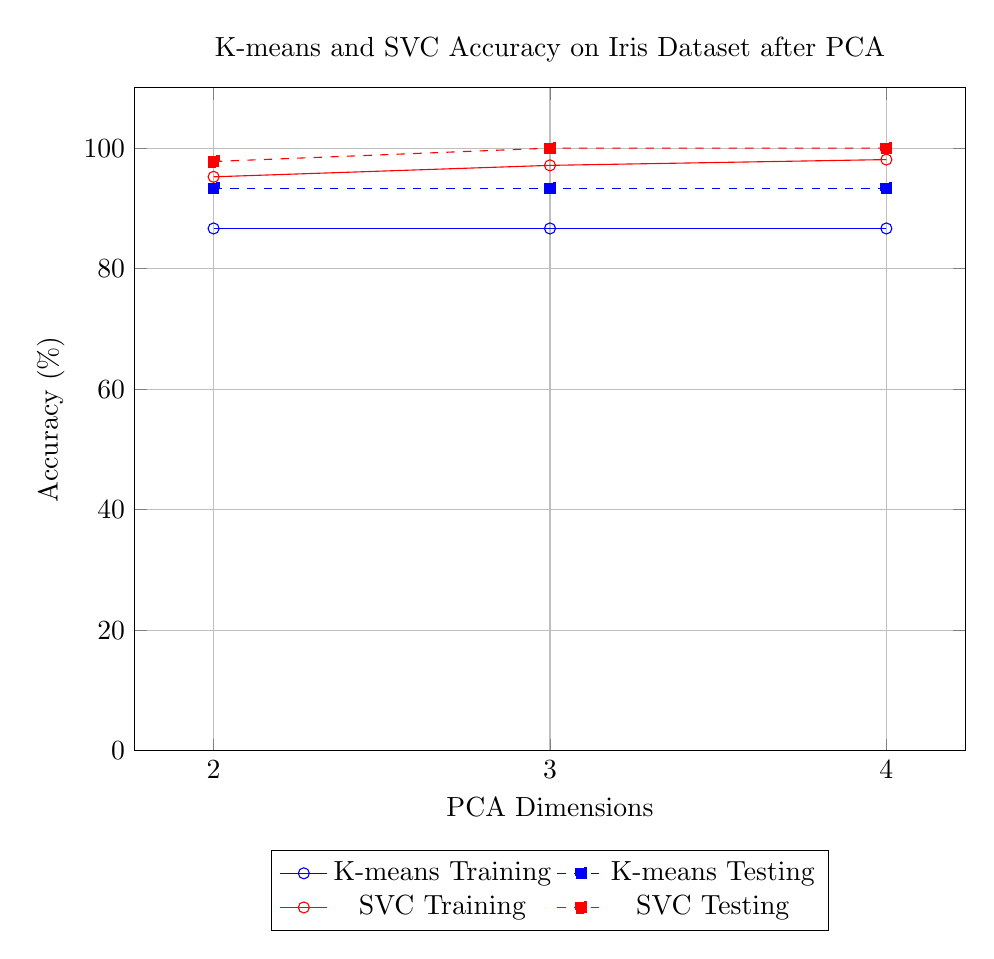
\begin{tikzpicture}
\begin{axis}[
    width=\textwidth, 
    height=10cm, 
    xlabel={PCA Dimensions}, 
    ylabel={Accuracy (\%)}, 
    xtick={4, 3, 2}, % Explicitly set the positions for PCA dimensions
    xticklabels={4, 3, 2}, % Corresponding labels
    ymin=0, ymax=110,
    grid=both, 
    legend style={at={(0.5,-0.15)}, anchor=north, legend columns=2},
    title={K-means and SVC Accuracy on Iris Dataset after PCA},
    enlarge x limits={abs=1cm},
]
% K-means Training and Testing (Iris)
\addplot[mark=o, color=blue] coordinates {(4, 86.67) (3, 86.67) (2, 86.67)};
\addplot[mark=square*, color=blue, dashed] coordinates {(4, 93.33) (3, 93.33) (2, 93.33)};
% SVC Training and Testing (Iris)
\addplot[mark=o, color=red] coordinates {(4, 98.10) (3, 97.14) (2, 95.24)};
\addplot[mark=square*, color=red, dashed] coordinates {(4, 100.00) (3, 100.00) (2, 97.78)};
\legend{K-means Training, K-means Testing, SVC Training, SVC Testing}
\end{axis}
\end{tikzpicture}
\caption{K-means and SVC Accuracy on Iris Dataset (Training and Testing after PCA)}
\end{figure}

% MNIST Dataset Line Plot
\begin{figure}[h!]
\centering
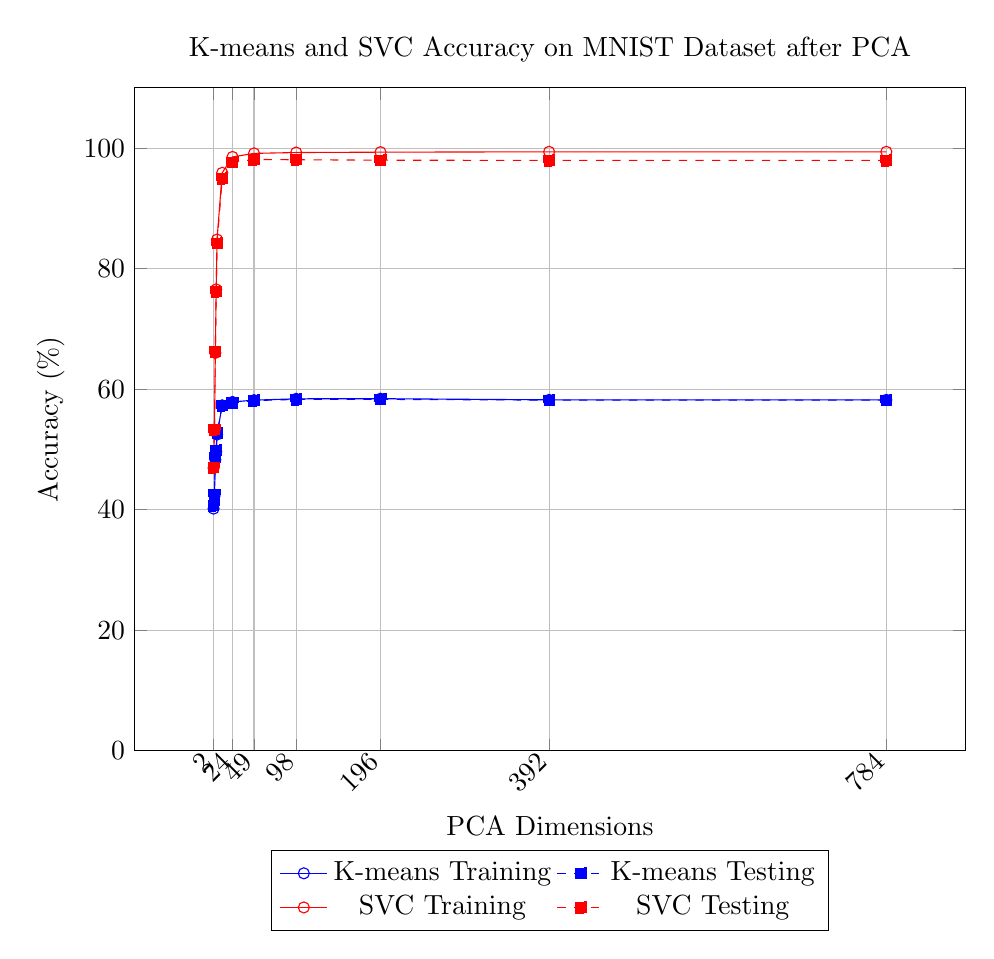
\begin{tikzpicture}
\begin{axis}[
    width=\textwidth, 
    height=10cm, 
    xlabel={PCA Dimensions}, 
    ylabel={Accuracy (\%)}, 
    xtick={784, 392, 196, 98, 49, 24, 2}, % Explicitly set positions for MNIST dimensions
    xticklabels={784, 392, 196, 98, 49, 24, 2}, % Corresponding labels
    ymin=0, ymax=110,
    grid=both, 
    legend style={at={(0.5,-0.15)}, anchor=north, legend columns=2},
    title={K-means and SVC Accuracy on MNIST Dataset after PCA},
    enlarge x limits={abs=1cm},
    x tick label style={rotate=45, anchor=east} % Rotating x-axis labels for better readability
]
% K-means Training and Testing (MNIST)
\addplot[mark=o, color=blue] coordinates {(784, 58.23) (392, 58.23) (196, 58.42) (98, 58.40) (49, 58.18) (24, 57.88) (12, 57.32) (6, 52.47) (5, 49.64) (4, 48.31) (3, 42.28) (2, 40.18)};
\addplot[mark=square*, color=blue, dashed] coordinates {(784, 58.18) (392, 58.19) (196, 58.31) (98, 58.30) (49, 58.11) (24, 57.71) (12, 57.23) (6, 52.70) (5, 49.90) (4, 48.68) (3, 42.49) (2, 40.67)};
% SVC Training and Testing (MNIST)
\addplot[mark=o, color=red] coordinates {(784, 99.39) (392, 99.39) (196, 99.33) (98, 99.27) (49, 99.13) (24, 98.54) (12, 95.90) (6, 84.83) (5, 76.55) (4, 66.02) (3, 53.21) (2, 46.92)};
\addplot[mark=square*, color=red, dashed] coordinates {(784, 97.96) (392, 97.96) (196, 98.00) (98, 98.07) (49, 98.12) (24, 97.65) (12, 94.96) (6, 84.22) (5, 76.19) (4, 66.22) (3, 53.27) (2, 46.98)};
\legend{K-means Training, K-means Testing, SVC Training, SVC Testing}
\end{axis}
\end{tikzpicture}
\caption{K-means and SVC Accuracy on MNIST Dataset (Training and Testing after PCA)}
\end{figure}


% MNIST Dataset (PCA from 12 to 2 Dimensions)
\begin{figure}[h!]
\centering
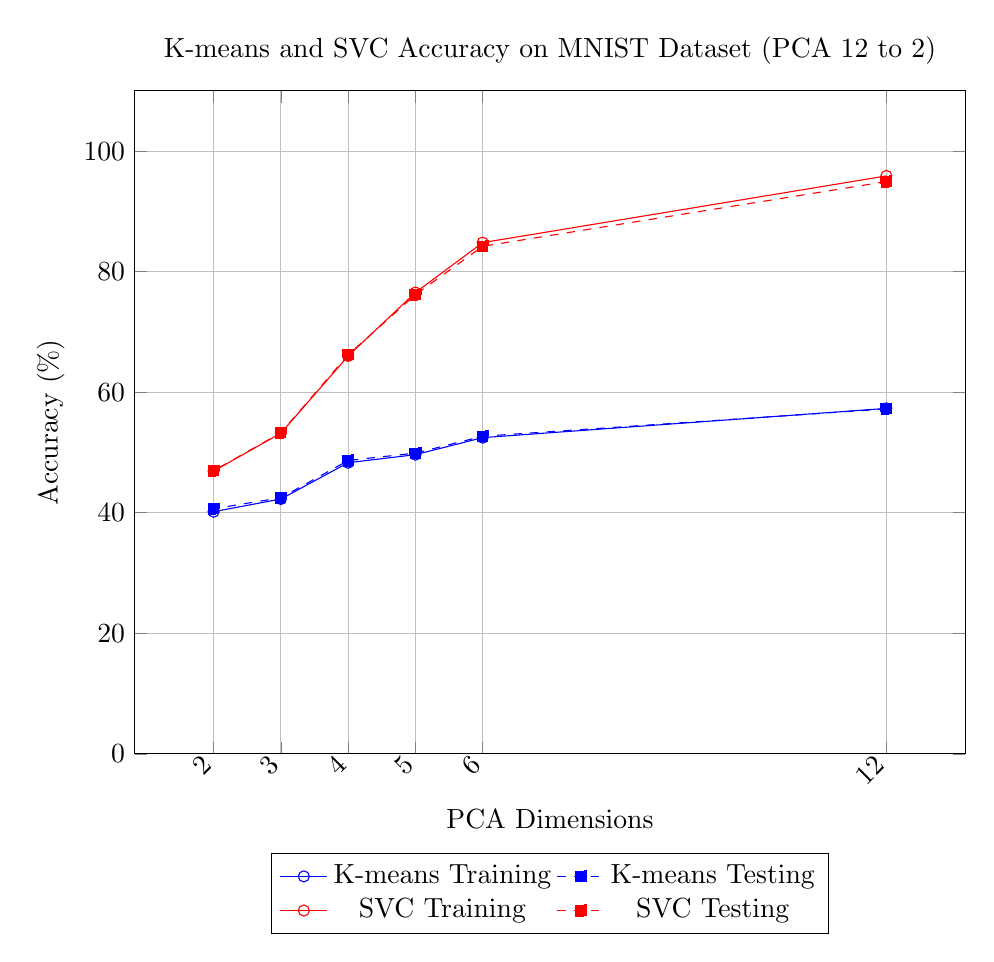
\begin{tikzpicture}
\begin{axis}[
    width=\textwidth, 
    height=10cm, 
    xlabel={PCA Dimensions}, 
    ylabel={Accuracy (\%)}, 
    xtick={12, 6, 5, 4, 3, 2}, % Explicitly set positions for PCA dimensions from 12 to 2
    xticklabels={12, 6, 5, 4, 3, 2}, % Corresponding labels for PCA dimensions
    ymin=0, ymax=110,
    grid=both, 
    legend style={at={(0.5,-0.15)}, anchor=north, legend columns=2},
    title={K-means and SVC Accuracy on MNIST Dataset (PCA 12 to 2)},
    enlarge x limits={abs=1cm},
    x tick label style={rotate=45, anchor=east} % Rotating x-axis labels for better readability
]
% K-means Training and Testing (MNIST)
\addplot[mark=o, color=blue] coordinates {(12, 57.32) (6, 52.47) (5, 49.64) (4, 48.31) (3, 42.28) (2, 40.18)};
\addplot[mark=square*, color=blue, dashed] coordinates {(12, 57.23) (6, 52.70) (5, 49.90) (4, 48.68) (3, 42.49) (2, 40.67)};
% SVC Training and Testing (MNIST)
\addplot[mark=o, color=red] coordinates {(12, 95.90) (6, 84.83) (5, 76.55) (4, 66.02) (3, 53.21) (2, 46.92)};
\addplot[mark=square*, color=red, dashed] coordinates {(12, 94.96) (6, 84.22) (5, 76.19) (4, 66.22) (3, 53.27) (2, 46.98)};
\legend{K-means Training, K-means Testing, SVC Training, SVC Testing}
\end{axis}
\end{tikzpicture}
\caption{K-means and SVC Accuracy on MNIST Dataset (PCA 12 to 2)}
\end{figure}

\end{document}
